\section{Introduction and Project Scope}
\label{sec:introduction}

\subsection{Project 2 objectives}
Project 2 develops a physics-based Falcon 9 simulator and a navigation system driven by simulated sensor measurements. Forces, moments, changing mass properties, and numerical integration generate the vehicle motion; the navigation algorithm estimates states from imperfect observations of that motion. The course identifies this environment as the computational foundation for guidance design in Project 3 and integrated control in Project 4 \cite[slides 2--4]{project2}.

The assignment covers equations of motion and coordinate systems, gravity and atmosphere, propulsion and aerodynamics, mass/inertia variation, configuration changes, and estimation of position, velocity, attitude, and angular velocity. Its validation requirement combines representative flight phases, public flight-data comparisons, and navigation-error analysis \cite[slides 4--6]{project2}. Accordingly, the report distinguishes physical-model verification, agreement with external flight evidence, and estimation error relative to simulation truth. These comparisons establish different aspects of the simulator's credibility.

\subsection{CRS-10 selection and vehicle configuration}
CRS-10 is SpaceX's tenth contracted Dragon cargo-resupply mission to the International Space Station. The official mission material identifies a Falcon 9/Dragon launch from Launch Complex 39A, first-stage recovery at Landing Zone 1, and an approximate sequence of cutoff, separation, and restart events \cite{nasacrs10press}. The public technical webcast and its published ascent digitization provide an accessible reference for a quantitative comparison \cite{crs10webcast,crs10telemetry}.

The mission exercises three connected trajectory segments: common-stack ascent, first-stage return, and upper-stage continuation. It therefore tests configuration changes and inherited states as well as continuous motion. The Dragon payload also fixes the configuration choice: the model carries one loaded Dragon/trunk assembly rather than a generic satellite and fairing. NASA's $2490\,\mathrm{kg}$ cargo inventory is a subset of that loaded assembly, not its total mass \cite{nasacrs10overview}.

Figure~\ref{fig:crs10-context} identifies the selected hardware and official mission document. The press kit supplies mission context and approximate preflight timing; generic Falcon user guides supply supplementary geometry and operating-point evidence with their configuration/date limitations. Internal dimensions and mass properties require the evidence-qualified modeling described in the vehicle chapter.

\begin{figure}[!htbp]
\centering
\begin{minipage}[c]{0.57\linewidth}
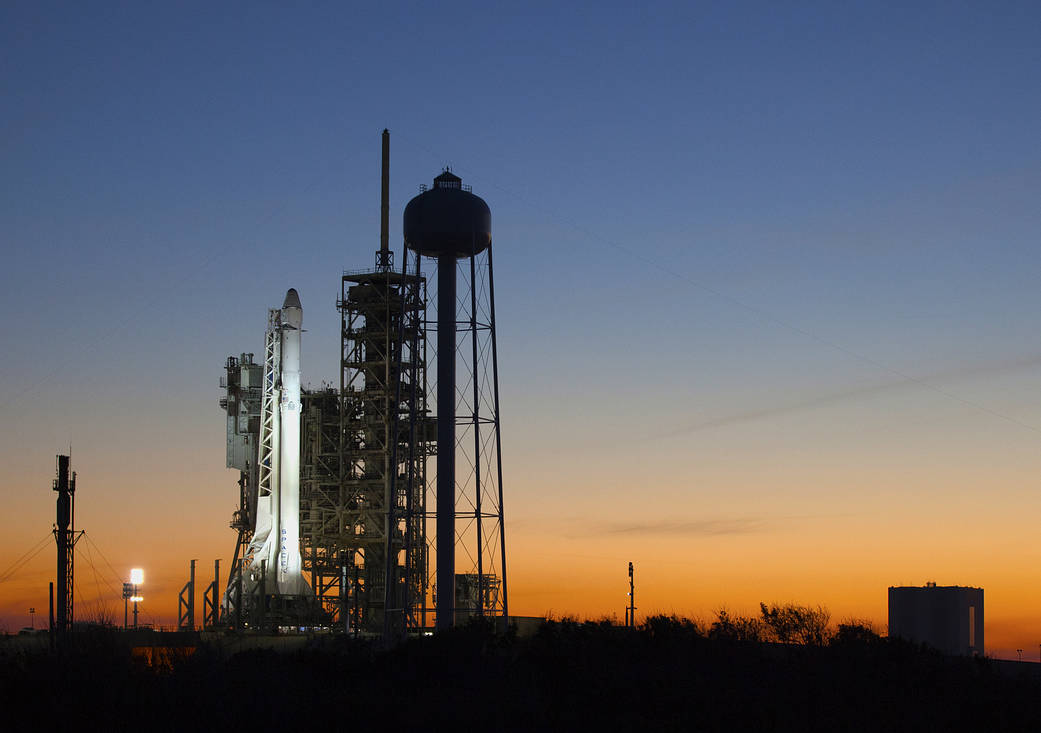
\includegraphics[width=\linewidth]{images/crs10_pad_nasa.jpg}
\end{minipage}\hfill
\begin{minipage}[c]{0.39\linewidth}
\centering
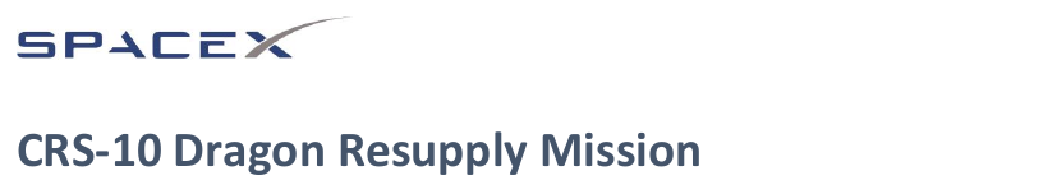
\includegraphics[width=\linewidth]{images/crs10_presskit_header.pdf}\\[1ex]
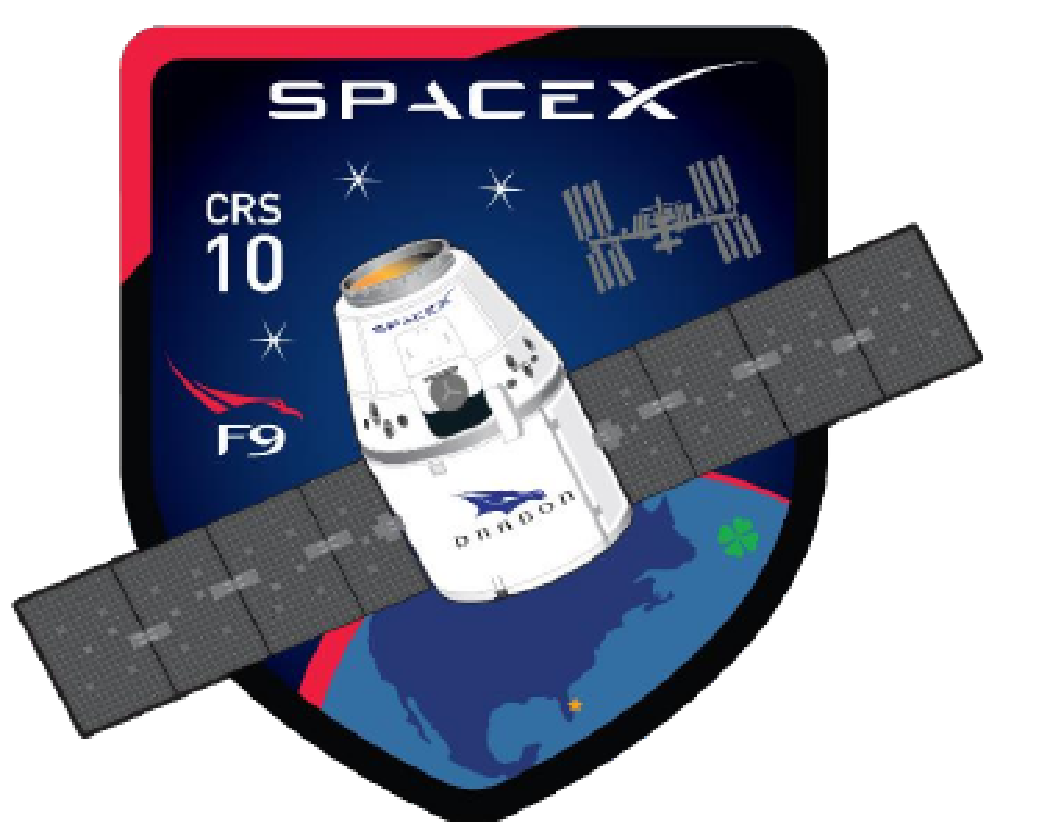
\includegraphics[width=0.60\linewidth]{images/crs10_mission_patch.pdf}
\end{minipage}
\caption{CRS-10 reference configuration. Left: Falcon 9 and Dragon at LC-39A before launch, NASA/Glenn Benson \cite{nasacrs10photo}. Right: header and mission-patch excerpts from the official SpaceX press kit \cite{nasacrs10press}. The images identify the hardware and source; they do not determine the internal mass distribution.}
\label{fig:crs10-context}
\end{figure}

\clearpage
\subsection{Simulation and validation scope}
The initial vehicle contains both stages and the loaded Dragon assembly. At separation, a conservative state map creates two children. The first stage proceeds through boostback, coast, entry burn, aerodynamic descent, landing burn, and first geometric contact. The upper child retains Dragon and continues under its own engine and attitude commands. Both children inherit the propagated separation state; a separately selected descent checkpoint does not create the full-return trajectory.

Flight commands provide a repeatable scenario for exercising the physical models. Scheduled reference times are distinguished from state-triggered return conditions, and project-designed return commands are classified as assumptions. The upper continuation demonstrates independent propagation rather than validated orbital insertion. First-stage navigation propagates its own quaternion from noisy gyros in a multiplicative extended Kalman filter (MEKF) with GNSS/LiDAR updates. A simulated star tracker supplies gated attitude observations; acceptance is checked per run. Physical attitude supplies sensor generation, an assumed initial alignment, and the evaluation reference; it is not continuously supplied to the active estimator.

External trajectory comparison uses the retained video-derived ascent observations over approximately $0$--$140\,\mathrm{s}$. Their classification is E: they are digitized public readouts, not released onboard telemetry. The ascent operating point and pitch timescale were adjusted using the same record, so their agreement is calibration evidence. Model-level tests, continuous state transfer, return/upper trajectories, and navigation errors provide additional evidence with their own stated assumptions. Navigation error against the simulator's truth does not by itself establish the accuracy of the physical vehicle model.
